\documentclass[twoside]{book}

% Packages required by doxygen
\usepackage{fixltx2e}
\usepackage{calc}
\usepackage{doxygen}
\usepackage[export]{adjustbox} % also loads graphicx
\usepackage{graphicx}
\usepackage[utf8]{inputenc}
\usepackage{makeidx}
\usepackage{multicol}
\usepackage{multirow}
\PassOptionsToPackage{warn}{textcomp}
\usepackage{textcomp}
\usepackage[nointegrals]{wasysym}
\usepackage[table]{xcolor}

% NLS support packages
\usepackage[spanish]{babel}
% Font selection
\usepackage[T1]{fontenc}
\usepackage[scaled=.90]{helvet}
\usepackage{courier}
\usepackage{amssymb}
\usepackage{sectsty}
\renewcommand{\familydefault}{\sfdefault}
\allsectionsfont{%
  \fontseries{bc}\selectfont%
  \color{darkgray}%
}
\renewcommand{\DoxyLabelFont}{%
  \fontseries{bc}\selectfont%
  \color{darkgray}%
}
\newcommand{\+}{\discretionary{\mbox{\scriptsize$\hookleftarrow$}}{}{}}

% Page & text layout
\usepackage{geometry}
\geometry{%
  a4paper,%
  top=2.5cm,%
  bottom=2.5cm,%
  left=2.5cm,%
  right=2.5cm%
}
\tolerance=750
\hfuzz=15pt
\hbadness=750
\setlength{\emergencystretch}{15pt}
\setlength{\parindent}{0cm}
\setlength{\parskip}{0.2cm}
\makeatletter
\renewcommand{\paragraph}{%
  \@startsection{paragraph}{4}{0ex}{-1.0ex}{1.0ex}{%
    \normalfont\normalsize\bfseries\SS@parafont%
  }%
}
\renewcommand{\subparagraph}{%
  \@startsection{subparagraph}{5}{0ex}{-1.0ex}{1.0ex}{%
    \normalfont\normalsize\bfseries\SS@subparafont%
  }%
}
\makeatother

% Headers & footers
\usepackage{fancyhdr}
\pagestyle{fancyplain}
\fancyhead[LE]{\fancyplain{}{\bfseries\thepage}}
\fancyhead[CE]{\fancyplain{}{}}
\fancyhead[RE]{\fancyplain{}{\bfseries\leftmark}}
\fancyhead[LO]{\fancyplain{}{\bfseries\rightmark}}
\fancyhead[CO]{\fancyplain{}{}}
\fancyhead[RO]{\fancyplain{}{\bfseries\thepage}}
\fancyfoot[LE]{\fancyplain{}{}}
\fancyfoot[CE]{\fancyplain{}{}}
\fancyfoot[RE]{\fancyplain{}{\bfseries\scriptsize Generado el Miércoles, 26 de Abril de 2017 10\+:55\+:06 para Practica P\+R\+O2 por Doxygen }}
\fancyfoot[LO]{\fancyplain{}{\bfseries\scriptsize Generado el Miércoles, 26 de Abril de 2017 10\+:55\+:06 para Practica P\+R\+O2 por Doxygen }}
\fancyfoot[CO]{\fancyplain{}{}}
\fancyfoot[RO]{\fancyplain{}{}}
\renewcommand{\footrulewidth}{0.4pt}
\renewcommand{\chaptermark}[1]{%
  \markboth{#1}{}%
}
\renewcommand{\sectionmark}[1]{%
  \markright{\thesection\ #1}%
}

% Indices & bibliography
\usepackage{natbib}
\usepackage[titles]{tocloft}
\setcounter{tocdepth}{3}
\setcounter{secnumdepth}{5}
\makeindex

% Hyperlinks (required, but should be loaded last)
\usepackage{ifpdf}
\ifpdf
  \usepackage[pdftex,pagebackref=true]{hyperref}
\else
  \usepackage[ps2pdf,pagebackref=true]{hyperref}
\fi
\hypersetup{%
  colorlinks=true,%
  linkcolor=blue,%
  citecolor=blue,%
  unicode%
}

% Custom commands
\newcommand{\clearemptydoublepage}{%
  \newpage{\pagestyle{empty}\cleardoublepage}%
}


%===== C O N T E N T S =====

\begin{document}

% Titlepage & ToC
\hypersetup{pageanchor=false,
             bookmarks=true,
             bookmarksnumbered=true,
             pdfencoding=unicode
            }
\pagenumbering{roman}
\begin{titlepage}
\vspace*{7cm}
\begin{center}%
{\Large Practica P\+R\+O2 \\[1ex]\large 25-\/abr-\/2017 }\\
\vspace*{1cm}
{\large Generado por Doxygen 1.8.9.1}\\
\vspace*{0.5cm}
{\small Miércoles, 26 de Abril de 2017 10:55:06}\\
\end{center}
\end{titlepage}
\clearemptydoublepage
\tableofcontents
\clearemptydoublepage
\pagenumbering{arabic}
\hypersetup{pageanchor=true}

%--- Begin generated contents ---
\chapter{Índice de clases}
\section{Lista de clases}
Lista de las clases, estructuras, uniones e interfaces con una breve descripción\+:\begin{DoxyCompactList}
\item\contentsline{section}{\hyperlink{class_arbol}{Arbol} }{\pageref{class_arbol}}{}
\item\contentsline{section}{\hyperlink{classarbol}{arbol} \\*Arbre genealogic afegit al sistema }{\pageref{classarbol}}{}
\item\contentsline{section}{\hyperlink{class_individu}{Individu} }{\pageref{class_individu}}{}
\item\contentsline{section}{\hyperlink{classindividu}{individu} \\*Representa un individu }{\pageref{classindividu}}{}
\item\contentsline{section}{\hyperlink{classpar__cromosmas}{par\+\_\+cromosmas} \\*Representa un parell de cromosmes }{\pageref{classpar__cromosmas}}{}
\item\contentsline{section}{\hyperlink{class_par___cromosmas}{Par\+\_\+\+Cromosmas} }{\pageref{class_par___cromosmas}}{}
\item\contentsline{section}{\hyperlink{class_poblacio}{Poblacio} }{\pageref{class_poblacio}}{}
\item\contentsline{section}{\hyperlink{classpoblacio}{poblacio} \\*Població representada per els individus afegits al sistema }{\pageref{classpoblacio}}{}
\end{DoxyCompactList}

\chapter{Indice de archivos}
\section{Lista de archivos}
Lista de todos los archivos con descripciones breves\+:\begin{DoxyCompactList}
\item\contentsline{section}{\hyperlink{arbol_8hh}{arbol.\+hh} \\*Classe \hyperlink{class_arbol}{Arbol} }{\pageref{arbol_8hh}}{}
\item\contentsline{section}{\hyperlink{individuo_8hh}{individuo.\+hh} }{\pageref{individuo_8hh}}{}
\item\contentsline{section}{\hyperlink{main_8cc}{main.\+cc} }{\pageref{main_8cc}}{}
\item\contentsline{section}{\hyperlink{par__cromosomas_8hh}{par\+\_\+cromosomas.\+hh} }{\pageref{par__cromosomas_8hh}}{}
\item\contentsline{section}{\hyperlink{poblacio_8hh}{poblacio.\+hh} \\*Classe \hyperlink{class_poblacio}{Poblacio} }{\pageref{poblacio_8hh}}{}
\end{DoxyCompactList}

\chapter{Documentación de las clases}
\hypertarget{class_arbol}{}\section{Referencia de la Clase Arbol}
\label{class_arbol}\index{Arbol@{Arbol}}
\subsection*{Métodos públicos}
\begin{DoxyCompactItemize}
\item 
void \hyperlink{class_arbol_a09980b861e2d8e4f3b1ac4f9ac13fb65}{escribir\+\_\+arbol\+\_\+genealogico} (string \hyperlink{classindividu}{individu})
\begin{DoxyCompactList}\small\item\em Escriu el arbre genealogic de l\textquotesingle{}individu. \end{DoxyCompactList}\item 
void a \hyperlink{class_arbol_a6d0fc9bf894ce3c644917298c4cd5390}{completar\+\_\+arbol\+\_\+genealogico} ()
\begin{DoxyCompactList}\small\item\em Completa el nostre arbre parcial amb els individus de la seva familia que tenim registrat al sistema. \end{DoxyCompactList}\item 
bool \hyperlink{class_arbol_a97e4cf3113d3ea3c04fbd49fa6871b1a}{es\+\_\+parcial} ()
\begin{DoxyCompactList}\small\item\em Ens indica si l\textquotesingle{}arbre genealogic es un arbre parcial. \end{DoxyCompactList}\end{DoxyCompactItemize}


\subsection{Descripción detallada}


Definición en la línea 16 del archivo arbol.\+hh.



\subsection{Documentación de las funciones miembro}
\hypertarget{class_arbol_a09980b861e2d8e4f3b1ac4f9ac13fb65}{}\index{Arbol@{Arbol}!escribir\+\_\+arbol\+\_\+genealogico@{escribir\+\_\+arbol\+\_\+genealogico}}
\index{escribir\+\_\+arbol\+\_\+genealogico@{escribir\+\_\+arbol\+\_\+genealogico}!Arbol@{Arbol}}
\subsubsection[{escribir\+\_\+arbol\+\_\+genealogico}]{\setlength{\rightskip}{0pt plus 5cm}void Arbol\+::escribir\+\_\+arbol\+\_\+genealogico (
\begin{DoxyParamCaption}
\item[{string}]{individu}
\end{DoxyParamCaption}
)}\label{class_arbol_a09980b861e2d8e4f3b1ac4f9ac13fb65}


Escriu el arbre genealogic de l\textquotesingle{}individu. 

\begin{DoxyPrecond}{Precondición}
\+: cert 
\end{DoxyPrecond}
\begin{DoxyPostcond}{Postcondición}
\+: ens escriu el arbre genealogic de l\textquotesingle{}individu, tenint com arrel el nostre individu. 
\end{DoxyPostcond}
\hypertarget{class_arbol_a6d0fc9bf894ce3c644917298c4cd5390}{}\index{Arbol@{Arbol}!completar\+\_\+arbol\+\_\+genealogico@{completar\+\_\+arbol\+\_\+genealogico}}
\index{completar\+\_\+arbol\+\_\+genealogico@{completar\+\_\+arbol\+\_\+genealogico}!Arbol@{Arbol}}
\subsubsection[{completar\+\_\+arbol\+\_\+genealogico}]{\setlength{\rightskip}{0pt plus 5cm}void a Arbol\+::completar\+\_\+arbol\+\_\+genealogico (
\begin{DoxyParamCaption}
{}
\end{DoxyParamCaption}
)}\label{class_arbol_a6d0fc9bf894ce3c644917298c4cd5390}


Completa el nostre arbre parcial amb els individus de la seva familia que tenim registrat al sistema. 

\begin{DoxyPrecond}{Precondición}
\+: cert 
\end{DoxyPrecond}
\begin{DoxyPostcond}{Postcondición}
\+: completa el arbre genealogic i ens diu si es parcial o no. 
\end{DoxyPostcond}
\hypertarget{class_arbol_a97e4cf3113d3ea3c04fbd49fa6871b1a}{}\index{Arbol@{Arbol}!es\+\_\+parcial@{es\+\_\+parcial}}
\index{es\+\_\+parcial@{es\+\_\+parcial}!Arbol@{Arbol}}
\subsubsection[{es\+\_\+parcial}]{\setlength{\rightskip}{0pt plus 5cm}bool Arbol\+::es\+\_\+parcial (
\begin{DoxyParamCaption}
{}
\end{DoxyParamCaption}
)}\label{class_arbol_a97e4cf3113d3ea3c04fbd49fa6871b1a}


Ens indica si l\textquotesingle{}arbre genealogic es un arbre parcial. 

\begin{DoxyPrecond}{Precondición}
\+: cert 
\end{DoxyPrecond}
\begin{DoxyPostcond}{Postcondición}
\+: es cert si l\textquotesingle{}arbre genaelogic es un arbre parcial. 
\end{DoxyPostcond}


La documentación para esta clase fue generada a partir del siguiente fichero\+:\begin{DoxyCompactItemize}
\item 
\hyperlink{arbol_8hh}{arbol.\+hh}\end{DoxyCompactItemize}

\hypertarget{classarbol}{}\section{Referencia de la Clase arbol}
\label{classarbol}\index{arbol@{arbol}}


Arbre genealogic afegit al sistema.  




\subsection{Descripción detallada}
Arbre genealogic afegit al sistema. 

La documentación para esta clase fue generada a partir del siguiente fichero\+:\begin{DoxyCompactItemize}
\item 
\hyperlink{arbol_8hh}{arbol.\+hh}\end{DoxyCompactItemize}

\hypertarget{class_individu}{}\section{Referencia de la Clase Individu}
\label{class_individu}\index{Individu@{Individu}}
\subsection*{Métodos públicos}
\begin{DoxyCompactItemize}
\item 
\hyperlink{class_individu_ab4416ff2c59e726dde0e43bc1789bcd1}{Individuo} ()
\begin{DoxyCompactList}\small\item\em Creació d\textquotesingle{}un individu. \end{DoxyCompactList}\item 
bool \hyperlink{class_individu_a65703ed67fc7ae3680f029ab299ca0c6}{genere} ()
\begin{DoxyCompactList}\small\item\em Comprova el gènere de l\textquotesingle{}individu, si és femení ens retorna fals, i si es masculí, cert. \end{DoxyCompactList}\item 
bool \hyperlink{class_individu_a6972de5e5cf268c724109924d4d9e1b1}{te\+\_\+pare} ()
\begin{DoxyCompactList}\small\item\em Comprova si l\textquotesingle{}individu té pare registrat al sistema. \end{DoxyCompactList}\item 
bool \hyperlink{class_individu_a611aebc390831b301a7369ea6dad4e46}{te\+\_\+mare} ()
\begin{DoxyCompactList}\small\item\em Comprova si l\textquotesingle{}individu té mare registrada al sistema. \end{DoxyCompactList}\item 
void \hyperlink{class_individu_a78858253fa55421333328229e52cdd83}{escribir\+\_\+genotipo} ()
\begin{DoxyCompactList}\small\item\em Escriu el genotip del individu seleccionat. \end{DoxyCompactList}\item 
void \hyperlink{class_individu_aea43bd466e3296757dc38f415181617c}{llegir\+\_\+comp\+\_\+gen\+\_\+i\+\_\+cromosomas\+\_\+sex} (int lx, int ly)
\begin{DoxyCompactList}\small\item\em Llegeix la composicio genetica i els cromosomes sexuals de un individu. \end{DoxyCompactList}\item 
void \hyperlink{class_individu_aa08ba93568733dcfeea8de98931e457f}{leer\+\_\+cromosomas\+\_\+n} (int posicion, int numero\+\_\+genes)
\begin{DoxyCompactList}\small\item\em Llegeix la posicio del vector de cromosomes i el numero de gens del mateix. \end{DoxyCompactList}\end{DoxyCompactItemize}


\subsection{Descripción detallada}


Definición en la línea 16 del archivo individuo.\+hh.



\subsection{Documentación de las funciones miembro}
\hypertarget{class_individu_ab4416ff2c59e726dde0e43bc1789bcd1}{}\index{Individu@{Individu}!Individuo@{Individuo}}
\index{Individuo@{Individuo}!Individu@{Individu}}
\subsubsection[{Individuo}]{\setlength{\rightskip}{0pt plus 5cm}Individu\+::\+Individuo (
\begin{DoxyParamCaption}
{}
\end{DoxyParamCaption}
)}\label{class_individu_ab4416ff2c59e726dde0e43bc1789bcd1}


Creació d\textquotesingle{}un individu. 

\hypertarget{class_individu_a65703ed67fc7ae3680f029ab299ca0c6}{}\index{Individu@{Individu}!genere@{genere}}
\index{genere@{genere}!Individu@{Individu}}
\subsubsection[{genere}]{\setlength{\rightskip}{0pt plus 5cm}bool Individu\+::genere (
\begin{DoxyParamCaption}
{}
\end{DoxyParamCaption}
)}\label{class_individu_a65703ed67fc7ae3680f029ab299ca0c6}


Comprova el gènere de l\textquotesingle{}individu, si és femení ens retorna fals, i si es masculí, cert. 

\begin{DoxyPrecond}{Precondición}
\+: cert 
\end{DoxyPrecond}
\begin{DoxyPostcond}{Postcondición}
\+: ens retorna cert si l\textquotesingle{}individu és de gènere masculí i fals si es de gènere femení. 
\end{DoxyPostcond}
\hypertarget{class_individu_a6972de5e5cf268c724109924d4d9e1b1}{}\index{Individu@{Individu}!te\+\_\+pare@{te\+\_\+pare}}
\index{te\+\_\+pare@{te\+\_\+pare}!Individu@{Individu}}
\subsubsection[{te\+\_\+pare}]{\setlength{\rightskip}{0pt plus 5cm}bool Individu\+::te\+\_\+pare (
\begin{DoxyParamCaption}
{}
\end{DoxyParamCaption}
)}\label{class_individu_a6972de5e5cf268c724109924d4d9e1b1}


Comprova si l\textquotesingle{}individu té pare registrat al sistema. 

\begin{DoxyPrecond}{Precondición}
\+: cert 
\end{DoxyPrecond}
\begin{DoxyPostcond}{Postcondición}
\+: cert si el pare de l\textquotesingle{}individu apareix en el sistema. 
\end{DoxyPostcond}
\hypertarget{class_individu_a611aebc390831b301a7369ea6dad4e46}{}\index{Individu@{Individu}!te\+\_\+mare@{te\+\_\+mare}}
\index{te\+\_\+mare@{te\+\_\+mare}!Individu@{Individu}}
\subsubsection[{te\+\_\+mare}]{\setlength{\rightskip}{0pt plus 5cm}bool Individu\+::te\+\_\+mare (
\begin{DoxyParamCaption}
{}
\end{DoxyParamCaption}
)}\label{class_individu_a611aebc390831b301a7369ea6dad4e46}


Comprova si l\textquotesingle{}individu té mare registrada al sistema. 

\begin{DoxyPrecond}{Precondición}
\+: cert 
\end{DoxyPrecond}
\begin{DoxyPostcond}{Postcondición}
\+: cert si la mare de l\textquotesingle{}individu apareix en el sistema. 
\end{DoxyPostcond}
\hypertarget{class_individu_a78858253fa55421333328229e52cdd83}{}\index{Individu@{Individu}!escribir\+\_\+genotipo@{escribir\+\_\+genotipo}}
\index{escribir\+\_\+genotipo@{escribir\+\_\+genotipo}!Individu@{Individu}}
\subsubsection[{escribir\+\_\+genotipo}]{\setlength{\rightskip}{0pt plus 5cm}void Individu\+::escribir\+\_\+genotipo (
\begin{DoxyParamCaption}
{}
\end{DoxyParamCaption}
)}\label{class_individu_a78858253fa55421333328229e52cdd83}


Escriu el genotip del individu seleccionat. 

\begin{DoxyPrecond}{Precondición}
\+: Al pi existeix el nostre individu. 
\end{DoxyPrecond}
\begin{DoxyPostcond}{Postcondición}
\+: Ens retorna de forma creixent de dentificador, el parell de cromosomes (primer els sexuals i després els N parells de cromosomes normals. 
\end{DoxyPostcond}
\hypertarget{class_individu_aea43bd466e3296757dc38f415181617c}{}\index{Individu@{Individu}!llegir\+\_\+comp\+\_\+gen\+\_\+i\+\_\+cromosomas\+\_\+sex@{llegir\+\_\+comp\+\_\+gen\+\_\+i\+\_\+cromosomas\+\_\+sex}}
\index{llegir\+\_\+comp\+\_\+gen\+\_\+i\+\_\+cromosomas\+\_\+sex@{llegir\+\_\+comp\+\_\+gen\+\_\+i\+\_\+cromosomas\+\_\+sex}!Individu@{Individu}}
\subsubsection[{llegir\+\_\+comp\+\_\+gen\+\_\+i\+\_\+cromosomas\+\_\+sex}]{\setlength{\rightskip}{0pt plus 5cm}void Individu\+::llegir\+\_\+comp\+\_\+gen\+\_\+i\+\_\+cromosomas\+\_\+sex (
\begin{DoxyParamCaption}
\item[{int}]{lx, }
\item[{int}]{ly}
\end{DoxyParamCaption}
)}\label{class_individu_aea43bd466e3296757dc38f415181617c}


Llegeix la composicio genetica i els cromosomes sexuals de un individu. 

\begin{DoxyPrecond}{Precondición}
\+: cert 
\end{DoxyPrecond}
\begin{DoxyPostcond}{Postcondición}
\+: Llegeix la composicio genetica i els cromosomes sexuals de un individu 
\end{DoxyPostcond}
\hypertarget{class_individu_aa08ba93568733dcfeea8de98931e457f}{}\index{Individu@{Individu}!leer\+\_\+cromosomas\+\_\+n@{leer\+\_\+cromosomas\+\_\+n}}
\index{leer\+\_\+cromosomas\+\_\+n@{leer\+\_\+cromosomas\+\_\+n}!Individu@{Individu}}
\subsubsection[{leer\+\_\+cromosomas\+\_\+n}]{\setlength{\rightskip}{0pt plus 5cm}void Individu\+::leer\+\_\+cromosomas\+\_\+n (
\begin{DoxyParamCaption}
\item[{int}]{posicion, }
\item[{int}]{numero\+\_\+genes}
\end{DoxyParamCaption}
)}\label{class_individu_aa08ba93568733dcfeea8de98931e457f}


Llegeix la posicio del vector de cromosomes i el numero de gens del mateix. 

\begin{DoxyPrecond}{Precondición}
\+: cert 
\end{DoxyPrecond}
\begin{DoxyPostcond}{Postcondición}
\+: Llegeix la posicio del vector de cromosomes i el numero de gens del mateix 
\end{DoxyPostcond}


La documentación para esta clase fue generada a partir del siguiente fichero\+:\begin{DoxyCompactItemize}
\item 
\hyperlink{individuo_8hh}{individuo.\+hh}\end{DoxyCompactItemize}

\hypertarget{classindividu}{}\section{Referencia de la Clase individu}
\label{classindividu}\index{individu@{individu}}


Representa un individu.  




\subsection{Descripción detallada}
Representa un individu. 

La documentación para esta clase fue generada a partir del siguiente fichero\+:\begin{DoxyCompactItemize}
\item 
\hyperlink{individuo_8hh}{individuo.\+hh}\end{DoxyCompactItemize}

\hypertarget{classpar__cromosmas}{}\section{Referencia de la Clase par\+\_\+cromosmas}
\label{classpar__cromosmas}\index{par\+\_\+cromosmas@{par\+\_\+cromosmas}}


Representa un parell de cromosmes.  




\subsection{Descripción detallada}
Representa un parell de cromosmes. 

La documentación para esta clase fue generada a partir del siguiente fichero\+:\begin{DoxyCompactItemize}
\item 
\hyperlink{par__cromosomas_8hh}{par\+\_\+cromosomas.\+hh}\end{DoxyCompactItemize}

\hypertarget{class_par___cromosmas}{}\section{Referencia de la Clase Par\+\_\+\+Cromosmas}
\label{class_par___cromosmas}\index{Par\+\_\+\+Cromosmas@{Par\+\_\+\+Cromosmas}}
\subsection*{Métodos públicos}
\begin{DoxyCompactItemize}
\item 
void \hyperlink{class_par___cromosmas_a60fb703c5cbe7efb659bb416a363113c}{leer\+\_\+cromosmas\+\_\+n} (vector$<$ int $>$ l, int N)
\begin{DoxyCompactList}\small\item\em Llegeix el parell de cromosomes normals que toca segons la posició del vector en la que estem. \end{DoxyCompactList}\item 
void \hyperlink{class_par___cromosmas_a7857ea8f3ec852de93fac2f0963ceee1}{leer\+\_\+cromosmas\+\_\+sex} (int lx, ly)
\begin{DoxyCompactList}\small\item\em Llegeix el parell de cromosomes sexuals x. \end{DoxyCompactList}\item 
void \hyperlink{class_par___cromosmas_ad3a3c1e5cbcc3007862c0cb857647725}{reproduccio\+\_\+cromosomes} (vector$<$ int $>$ cromosomes\+\_\+pare, vector$<$ int $>$ cromosomes\+\_\+mare, int k)
\begin{DoxyCompactList}\small\item\em Produïrà els cromosomes del nou individu segons els cromosomes sexuals del pare i mare i el punt de tall. \end{DoxyCompactList}\end{DoxyCompactItemize}


\subsection{Descripción detallada}


Definición en la línea 16 del archivo par\+\_\+cromosomas.\+hh.



\subsection{Documentación de las funciones miembro}
\hypertarget{class_par___cromosmas_a60fb703c5cbe7efb659bb416a363113c}{}\index{Par\+\_\+\+Cromosmas@{Par\+\_\+\+Cromosmas}!leer\+\_\+cromosmas\+\_\+n@{leer\+\_\+cromosmas\+\_\+n}}
\index{leer\+\_\+cromosmas\+\_\+n@{leer\+\_\+cromosmas\+\_\+n}!Par\+\_\+\+Cromosmas@{Par\+\_\+\+Cromosmas}}
\subsubsection[{leer\+\_\+cromosmas\+\_\+n}]{\setlength{\rightskip}{0pt plus 5cm}void Par\+\_\+\+Cromosmas\+::leer\+\_\+cromosmas\+\_\+n (
\begin{DoxyParamCaption}
\item[{vector$<$ int $>$}]{l, }
\item[{int}]{N}
\end{DoxyParamCaption}
)}\label{class_par___cromosmas_a60fb703c5cbe7efb659bb416a363113c}


Llegeix el parell de cromosomes normals que toca segons la posició del vector en la que estem. 

\begin{DoxyPrecond}{Precondición}
\+: cert 
\end{DoxyPrecond}
\begin{DoxyPostcond}{Postcondición}
\+: ens llegeix el parell de cormosomes normals 
\end{DoxyPostcond}
\hypertarget{class_par___cromosmas_a7857ea8f3ec852de93fac2f0963ceee1}{}\index{Par\+\_\+\+Cromosmas@{Par\+\_\+\+Cromosmas}!leer\+\_\+cromosmas\+\_\+sex@{leer\+\_\+cromosmas\+\_\+sex}}
\index{leer\+\_\+cromosmas\+\_\+sex@{leer\+\_\+cromosmas\+\_\+sex}!Par\+\_\+\+Cromosmas@{Par\+\_\+\+Cromosmas}}
\subsubsection[{leer\+\_\+cromosmas\+\_\+sex}]{\setlength{\rightskip}{0pt plus 5cm}void Par\+\_\+\+Cromosmas\+::leer\+\_\+cromosmas\+\_\+sex (
\begin{DoxyParamCaption}
\item[{int}]{lx, }
\item[{ly}]{}
\end{DoxyParamCaption}
)}\label{class_par___cromosmas_a7857ea8f3ec852de93fac2f0963ceee1}


Llegeix el parell de cromosomes sexuals x. 

\begin{DoxyPrecond}{Precondición}
\+: cert 
\end{DoxyPrecond}
\begin{DoxyPostcond}{Postcondición}
\+: ens llegeix el parell de cromosomes sexuals 
\end{DoxyPostcond}
\hypertarget{class_par___cromosmas_ad3a3c1e5cbcc3007862c0cb857647725}{}\index{Par\+\_\+\+Cromosmas@{Par\+\_\+\+Cromosmas}!reproduccio\+\_\+cromosomes@{reproduccio\+\_\+cromosomes}}
\index{reproduccio\+\_\+cromosomes@{reproduccio\+\_\+cromosomes}!Par\+\_\+\+Cromosmas@{Par\+\_\+\+Cromosmas}}
\subsubsection[{reproduccio\+\_\+cromosomes}]{\setlength{\rightskip}{0pt plus 5cm}void Par\+\_\+\+Cromosmas\+::reproduccio\+\_\+cromosomes (
\begin{DoxyParamCaption}
\item[{vector$<$ int $>$}]{cromosomes\+\_\+pare, }
\item[{vector$<$ int $>$}]{cromosomes\+\_\+mare, }
\item[{int}]{k}
\end{DoxyParamCaption}
)}\label{class_par___cromosmas_ad3a3c1e5cbcc3007862c0cb857647725}


Produïrà els cromosomes del nou individu segons els cromosomes sexuals del pare i mare i el punt de tall. 

\begin{DoxyPrecond}{Precondición}
\+: cert 
\end{DoxyPrecond}
\begin{DoxyPostcond}{Postcondición}
\+: Es crea el nou individu a partir del genotip dels pares. 
\end{DoxyPostcond}


La documentación para esta clase fue generada a partir del siguiente fichero\+:\begin{DoxyCompactItemize}
\item 
\hyperlink{par__cromosomas_8hh}{par\+\_\+cromosomas.\+hh}\end{DoxyCompactItemize}

\hypertarget{class_poblacio}{}\section{Referencia de la Clase Poblacio}
\label{class_poblacio}\index{Poblacio@{Poblacio}}
\subsection*{Métodos públicos}
\begin{DoxyCompactItemize}
\item 
void \hyperlink{class_poblacio_ac27c16bc83806f37ced94a4ca16dcde3}{escribir\+\_\+poblacion} () const 
\begin{DoxyCompactList}\small\item\em Escribe todos los individuos registrados en el sistema. \end{DoxyCompactList}\item 
void \hyperlink{class_poblacio_a4f0ee787d73f542b695bdb7640b0c19f}{anadir\+\_\+individuo} (const individuo \&i)
\begin{DoxyCompactList}\small\item\em Añade un individuo al sistema. \end{DoxyCompactList}\item 
void \hyperlink{class_poblacio_a2967d103f843c3566fb2a7e4f97e0552}{reproduccion\+\_\+sexual} (string nom\+\_\+pare, string nom\+\_\+mare, string nom\+\_\+fill)
\begin{DoxyCompactList}\small\item\em Produeix un nou individu donat un pare i una mare vàlids. \end{DoxyCompactList}\item 
Individuo \hyperlink{class_poblacio_a82e917e29d78fda03e1f94cc5deb028b}{buscar\+\_\+individuo} (string nom)
\begin{DoxyCompactList}\small\item\em Busca al map de poblacio l\textquotesingle{}individu seleccionat. \end{DoxyCompactList}\item 
bool \hyperlink{class_poblacio_ae9b6311a7f75edca20d9bdeaf82f2e5c}{existeix} (string nom\+\_\+individu)
\begin{DoxyCompactList}\small\item\em Comprova si l\textquotesingle{}individu ja està registrat al sistema. \end{DoxyCompactList}\item 
bool \hyperlink{class_poblacio_a56949cb9cd49b9e8b4a34046b232b2e6}{son\+\_\+germans} (string nom\+\_\+pare, string nom\+\_\+mare)
\begin{DoxyCompactList}\small\item\em Comprova si els dos individus son germans. \end{DoxyCompactList}\item 
bool \hyperlink{class_poblacio_a56baf60bde2953ed2b2069ae05b5971f}{son\+\_\+antecesors} (string nom\+\_\+pare, string nom\+\_\+mare)
\begin{DoxyCompactList}\small\item\em Comprova si algun individu es antecesor de l\textquotesingle{}altre. \end{DoxyCompactList}\end{DoxyCompactItemize}


\subsection{Descripción detallada}


Definición en la línea 18 del archivo poblacio.\+hh.



\subsection{Documentación de las funciones miembro}
\hypertarget{class_poblacio_ac27c16bc83806f37ced94a4ca16dcde3}{}\index{Poblacio@{Poblacio}!escribir\+\_\+poblacion@{escribir\+\_\+poblacion}}
\index{escribir\+\_\+poblacion@{escribir\+\_\+poblacion}!Poblacio@{Poblacio}}
\subsubsection[{escribir\+\_\+poblacion}]{\setlength{\rightskip}{0pt plus 5cm}void Poblacio\+::escribir\+\_\+poblacion (
\begin{DoxyParamCaption}
{}
\end{DoxyParamCaption}
) const}\label{class_poblacio_ac27c16bc83806f37ced94a4ca16dcde3}


Escribe todos los individuos registrados en el sistema. 

\begin{DoxyPrecond}{Precondición}
\+: cert. 
\end{DoxyPrecond}
\begin{DoxyPostcond}{Postcondición}
\+: escriu els 
\end{DoxyPostcond}
\hypertarget{class_poblacio_a4f0ee787d73f542b695bdb7640b0c19f}{}\index{Poblacio@{Poblacio}!anadir\+\_\+individuo@{anadir\+\_\+individuo}}
\index{anadir\+\_\+individuo@{anadir\+\_\+individuo}!Poblacio@{Poblacio}}
\subsubsection[{anadir\+\_\+individuo}]{\setlength{\rightskip}{0pt plus 5cm}void Poblacio\+::anadir\+\_\+individuo (
\begin{DoxyParamCaption}
\item[{const individuo \&}]{i}
\end{DoxyParamCaption}
)}\label{class_poblacio_a4f0ee787d73f542b695bdb7640b0c19f}


Añade un individuo al sistema. 

\begin{DoxyPrecond}{Precondición}
\+: L\textquotesingle{}individu no és al pi encara 
\end{DoxyPrecond}
\begin{DoxyPostcond}{Postcondición}
\+: s\textquotesingle{}ha afegit un nou individu al pi 
\end{DoxyPostcond}
\hypertarget{class_poblacio_a2967d103f843c3566fb2a7e4f97e0552}{}\index{Poblacio@{Poblacio}!reproduccion\+\_\+sexual@{reproduccion\+\_\+sexual}}
\index{reproduccion\+\_\+sexual@{reproduccion\+\_\+sexual}!Poblacio@{Poblacio}}
\subsubsection[{reproduccion\+\_\+sexual}]{\setlength{\rightskip}{0pt plus 5cm}void Poblacio\+::reproduccion\+\_\+sexual (
\begin{DoxyParamCaption}
\item[{string}]{nom\+\_\+pare, }
\item[{string}]{nom\+\_\+mare, }
\item[{string}]{nom\+\_\+fill}
\end{DoxyParamCaption}
)}\label{class_poblacio_a2967d103f843c3566fb2a7e4f97e0552}


Produeix un nou individu donat un pare i una mare vàlids. 

\begin{DoxyPrecond}{Precondición}
\+: Al pi existeixen el pare i la mare, però no el nou individu. 
\end{DoxyPrecond}
\begin{DoxyPostcond}{Postcondición}
\+: Es crea un nou individu. 
\end{DoxyPostcond}
\hypertarget{class_poblacio_a82e917e29d78fda03e1f94cc5deb028b}{}\index{Poblacio@{Poblacio}!buscar\+\_\+individuo@{buscar\+\_\+individuo}}
\index{buscar\+\_\+individuo@{buscar\+\_\+individuo}!Poblacio@{Poblacio}}
\subsubsection[{buscar\+\_\+individuo}]{\setlength{\rightskip}{0pt plus 5cm}Individuo Poblacio\+::buscar\+\_\+individuo (
\begin{DoxyParamCaption}
\item[{string}]{nom}
\end{DoxyParamCaption}
)}\label{class_poblacio_a82e917e29d78fda03e1f94cc5deb028b}


Busca al map de poblacio l\textquotesingle{}individu seleccionat. 

\begin{DoxyPrecond}{Precondición}
\+: Al pi existeix l\textquotesingle{}individu 
\end{DoxyPrecond}
\begin{DoxyPostcond}{Postcondición}
\+: Ens retorna el \hyperlink{class_individu}{Individu} 
\end{DoxyPostcond}
\hypertarget{class_poblacio_ae9b6311a7f75edca20d9bdeaf82f2e5c}{}\index{Poblacio@{Poblacio}!existeix@{existeix}}
\index{existeix@{existeix}!Poblacio@{Poblacio}}
\subsubsection[{existeix}]{\setlength{\rightskip}{0pt plus 5cm}bool Poblacio\+::existeix (
\begin{DoxyParamCaption}
\item[{string}]{nom\+\_\+individu}
\end{DoxyParamCaption}
)}\label{class_poblacio_ae9b6311a7f75edca20d9bdeaf82f2e5c}


Comprova si l\textquotesingle{}individu ja està registrat al sistema. 

\begin{DoxyPrecond}{Precondición}
\+: cert 
\end{DoxyPrecond}
\begin{DoxyPostcond}{Postcondición}
\+: cert si l\textquotesingle{}individu apareix registrat en el sistema. 
\end{DoxyPostcond}
\hypertarget{class_poblacio_a56949cb9cd49b9e8b4a34046b232b2e6}{}\index{Poblacio@{Poblacio}!son\+\_\+germans@{son\+\_\+germans}}
\index{son\+\_\+germans@{son\+\_\+germans}!Poblacio@{Poblacio}}
\subsubsection[{son\+\_\+germans}]{\setlength{\rightskip}{0pt plus 5cm}bool Poblacio\+::son\+\_\+germans (
\begin{DoxyParamCaption}
\item[{string}]{nom\+\_\+pare, }
\item[{string}]{nom\+\_\+mare}
\end{DoxyParamCaption}
)}\label{class_poblacio_a56949cb9cd49b9e8b4a34046b232b2e6}


Comprova si els dos individus son germans. 

\begin{DoxyPrecond}{Precondición}
\+: cert 
\end{DoxyPrecond}
\begin{DoxyPostcond}{Postcondición}
\+: ens retorna cert si els dons individus son germans (comparteixen pare i/o mare) 
\end{DoxyPostcond}
\hypertarget{class_poblacio_a56baf60bde2953ed2b2069ae05b5971f}{}\index{Poblacio@{Poblacio}!son\+\_\+antecesors@{son\+\_\+antecesors}}
\index{son\+\_\+antecesors@{son\+\_\+antecesors}!Poblacio@{Poblacio}}
\subsubsection[{son\+\_\+antecesors}]{\setlength{\rightskip}{0pt plus 5cm}bool Poblacio\+::son\+\_\+antecesors (
\begin{DoxyParamCaption}
\item[{string}]{nom\+\_\+pare, }
\item[{string}]{nom\+\_\+mare}
\end{DoxyParamCaption}
)}\label{class_poblacio_a56baf60bde2953ed2b2069ae05b5971f}


Comprova si algun individu es antecesor de l\textquotesingle{}altre. 

\begin{DoxyPrecond}{Precondición}
\+: cert 
\end{DoxyPrecond}
\begin{DoxyPostcond}{Postcondición}
\+: ens retorna cert si algun dels dos individus és antecesor de l\textquotesingle{}altre. 
\end{DoxyPostcond}


La documentación para esta clase fue generada a partir del siguiente fichero\+:\begin{DoxyCompactItemize}
\item 
\hyperlink{poblacio_8hh}{poblacio.\+hh}\end{DoxyCompactItemize}

\hypertarget{classpoblacio}{}\section{Referencia de la Clase poblacio}
\label{classpoblacio}\index{poblacio@{poblacio}}


Població representada per els individus afegits al sistema.  




\subsection{Descripción detallada}
Població representada per els individus afegits al sistema. 

La documentación para esta clase fue generada a partir del siguiente fichero\+:\begin{DoxyCompactItemize}
\item 
\hyperlink{poblacio_8hh}{poblacio.\+hh}\end{DoxyCompactItemize}

\chapter{Documentación de archivos}
\input{arbol_8hh}
\hypertarget{individuo_8hh}{}\section{Referencia del Archivo individuo.\+hh}
\label{individuo_8hh}\index{individuo.\+hh@{individuo.\+hh}}
Dependencia gráfica adjunta para individuo.\+hh\+:
\nopagebreak
\begin{figure}[H]
\begin{center}
\leavevmode
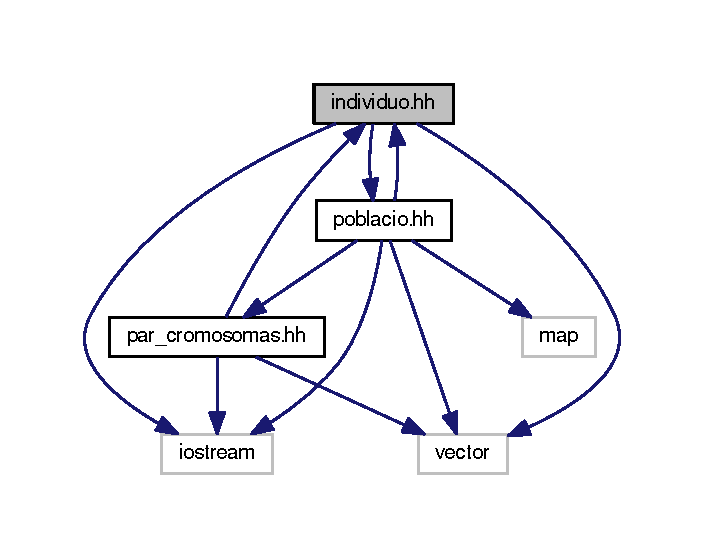
\includegraphics[width=338pt]{individuo_8hh__incl}
\end{center}
\end{figure}
\subsection*{Clases}
\begin{DoxyCompactItemize}
\item 
class \hyperlink{class_individu}{Individu}
\end{DoxyCompactItemize}

\hypertarget{main_8cc}{}\section{Referencia del Archivo main.\+cc}
\label{main_8cc}\index{main.\+cc@{main.\+cc}}
Dependencia gráfica adjunta para main.\+cc\+:
\nopagebreak
\begin{figure}[H]
\begin{center}
\leavevmode
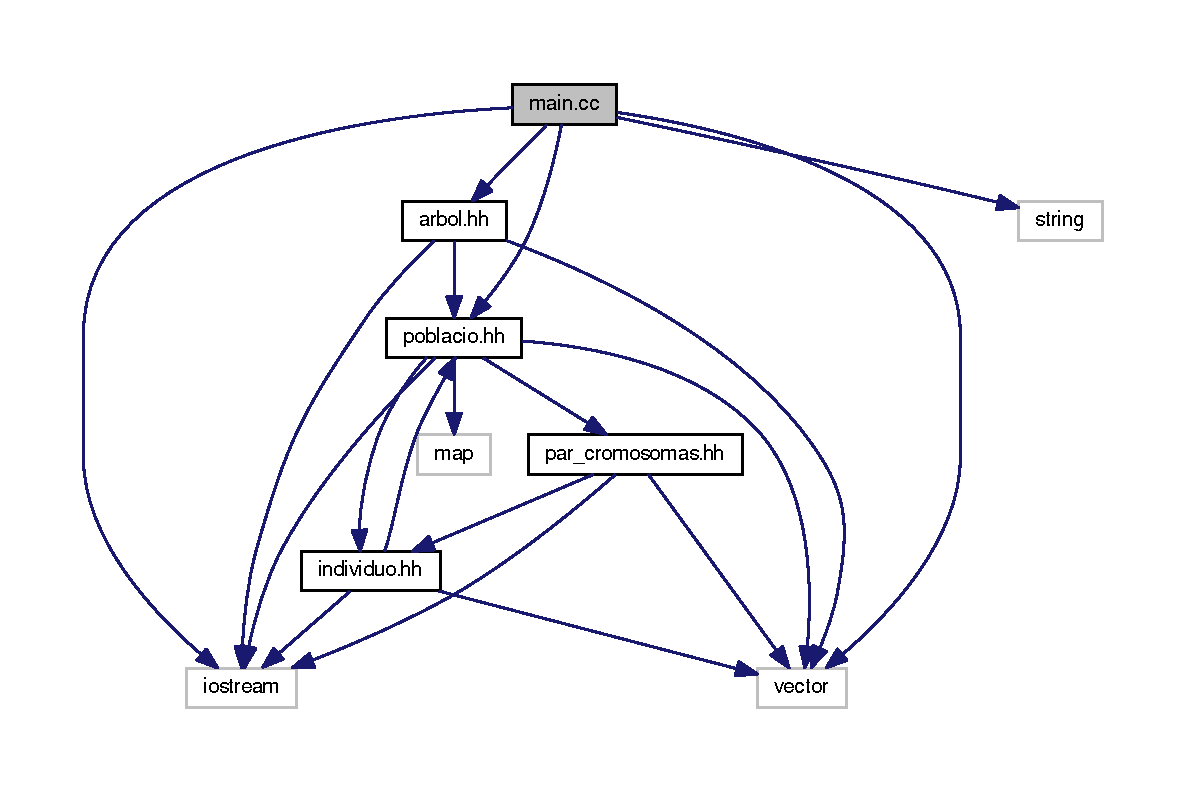
\includegraphics[width=350pt]{main_8cc__incl}
\end{center}
\end{figure}
\subsection*{Funciones}
\begin{DoxyCompactItemize}
\item 
int \hyperlink{main_8cc_ae66f6b31b5ad750f1fe042a706a4e3d4}{main} ()
\end{DoxyCompactItemize}


\subsection{Documentación de las funciones}
\hypertarget{main_8cc_ae66f6b31b5ad750f1fe042a706a4e3d4}{}\index{main.\+cc@{main.\+cc}!main@{main}}
\index{main@{main}!main.\+cc@{main.\+cc}}
\subsubsection[{main}]{\setlength{\rightskip}{0pt plus 5cm}int main (
\begin{DoxyParamCaption}
{}
\end{DoxyParamCaption}
)}\label{main_8cc_ae66f6b31b5ad750f1fe042a706a4e3d4}


Definición en la línea 8 del archivo main.\+cc.


\begin{DoxyCode}
8            \{
9     \textcolor{keywordtype}{int} N;
10     cin >> N;
11     \textcolor{keywordtype}{int} lx, ly;
12     vector <int> l(N+1);
13     \textcolor{keywordflow}{for} (\textcolor{keywordtype}{int} i = 0; i <= N; ++i) \{
14         cin >> l[i];
15     \}
16     cin >> lx >> ly;
17     \textcolor{keywordtype}{int} M;
18     cin >> M;
19     \textcolor{keywordtype}{string} nom\_individu;
20     \textcolor{keywordtype}{char} composicio\_genetica;
21     \hyperlink{classpoblacio}{poblacio} p;
22     \hyperlink{classarbol}{arbol} a;
23     \textcolor{keywordflow}{for} (\textcolor{keywordtype}{int} i = 0; i < M; ++i) \{
24         individuo indi(N);         \textcolor{comment}{//Pasar a individuo el numero de par de cromosomas}
25         cin >> nom\_individu;
26         indi.llegir\_comp\_gen\_i\_cromosomas\_sex(lx, ly);
27         \textcolor{keywordflow}{for} (\textcolor{keywordtype}{int} i = 0; i < N; ++i) \{
28             indi.leer\_cromosomas\_n(i,l[i]);       \textcolor{comment}{//posicion, numero de genes }
29         \}
30         p.anadir\_individuo(indi);
31     \}
32     \textcolor{keywordtype}{string} funciones;
33     \textcolor{keywordflow}{while} (cin >> funciones) \{
34         \textcolor{keywordflow}{if} (funciones == \textcolor{stringliteral}{"anadir\_indiviuo"}) \{
35             individuo indi(N);         \textcolor{comment}{//Pasar a individuo el numero de par de cromosomas}
36             cin >> nom\_individu;
37             indi.llegir\_comp\_gen\_i\_cromosomas\_sex(lx, ly);
38             \textcolor{keywordflow}{for} (\textcolor{keywordtype}{int} i = 0; i < N; ++i) \{
39                 indi.leer\_cromosomas\_n(i,l[i]);       \textcolor{comment}{//posicion, numero de genes }
40             \}
41                 
42             \textcolor{keywordflow}{if} (not p.existeix(nom\_individu)) p.anadir\_indiviuo(indi);
43             \textcolor{keywordflow}{else} cout << \textcolor{stringliteral}{"error"} << endl;
44         \}
45         
46         \textcolor{keywordflow}{else} \textcolor{keywordflow}{if} (funciones == \textcolor{stringliteral}{"reproduccion\_sexual"}) \{
47             \textcolor{keywordtype}{string} pare, mare, fill;
48             cin >> pare >> mare >> fill;                            
49             \textcolor{keywordflow}{if} (p.existeix(pare) and p.existeix(mare) and not p.existeix(fill)) \{
50                 Individuo indpare = p.buscar\_individuo(pare);
51                 Individuo indmare = p.buscar\_individuo(mare);
52                 \textcolor{keywordflow}{if} (indpare.genere() and not indmare.genere() and not p.son\_germans(pare, mare) and not p.
      son\_antecesors(pare, mare)) \{
53                         p.reproduccion\_sexual(pare, mare, fill);
54                 \}
55                 \textcolor{keywordflow}{else} cout << \textcolor{stringliteral}{"no es posible reproduccion sexual"} << endl;
56             \}
57             \textcolor{keywordflow}{else} cout << \textcolor{stringliteral}{"error"} << endl;
58         \}
59         
60         
61         \textcolor{keywordflow}{else} \textcolor{keywordflow}{if} (funciones == \textcolor{stringliteral}{"escribir\_arbol\_genealogico"}) \{
62             cin >> nom\_individu;
63             \textcolor{keywordflow}{if} (p.existeix(nom\_individu)) a.escribir\_arbol\_genealogico(nom\_individu);
64             \textcolor{keywordflow}{else} cout << \textcolor{stringliteral}{"error"} << endl;
65         \}
66         
67         \textcolor{keywordflow}{else} \textcolor{keywordflow}{if} (funciones == \textcolor{stringliteral}{"completar\_arbol\_genealogico"}) \{
68             a.completar\_arbol\_genealogico();
69             \textcolor{keywordflow}{if} (not a.completar\_arbol\_genealogico()) \{
70                 cout << \textcolor{stringliteral}{"no es arbol parcial"} << endl;
71             \}
72             
73         \}
74         
75         \textcolor{keywordflow}{else} \textcolor{keywordflow}{if} (funciones == \textcolor{stringliteral}{"escribir\_poblacion"}) \{
76             p.escribir\_poblacion();
77         \}
78         
79         \textcolor{keywordflow}{else} \textcolor{keywordflow}{if} (funciones == \textcolor{stringliteral}{"escribir\_genotipo"}) \{
80             cin >> nom\_individu;
81             \textcolor{keywordflow}{if} (p.existeix(nom\_individu)) \{
82                 individuo indi = p.buscar\_individuo(nom\_individu);
83                 indi.escribir\_genotipo();
84             \}
85             \textcolor{keywordflow}{else} cout << \textcolor{stringliteral}{"error"} << endl;
86         \}
87     \}
88 \}\end{DoxyCode}

\hypertarget{par__cromosomas_8hh}{}\section{Referencia del Archivo par\+\_\+cromosomas.\+hh}
\label{par__cromosomas_8hh}\index{par\+\_\+cromosomas.\+hh@{par\+\_\+cromosomas.\+hh}}
Dependencia gráfica adjunta para par\+\_\+cromosomas.\+hh\+:
\nopagebreak
\begin{figure}[H]
\begin{center}
\leavevmode
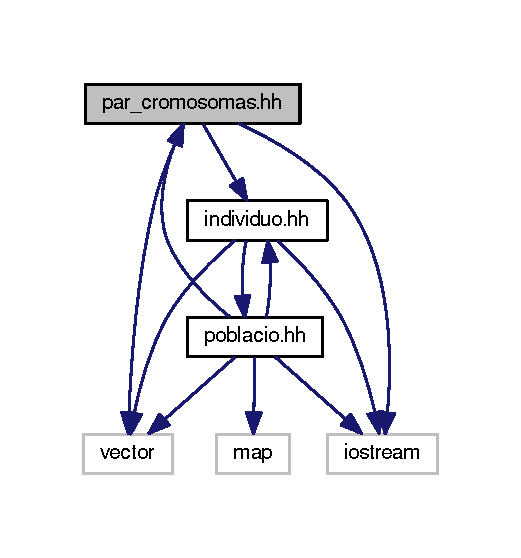
\includegraphics[width=250pt]{par__cromosomas_8hh__incl}
\end{center}
\end{figure}
\subsection*{Clases}
\begin{DoxyCompactItemize}
\item 
class \hyperlink{class_par___cromosmas}{Par\+\_\+\+Cromosmas}
\end{DoxyCompactItemize}
\subsection*{\textquotesingle{}defines\textquotesingle{}}
\begin{DoxyCompactItemize}
\item 
\#define \hyperlink{par__cromosomas_8hh_a76f8c8fb616d504ef7e9ff7b6d22af93}{P\+A\+R\+\_\+\+C\+R\+O\+M\+O\+S\+O\+M\+A\+S\+\_\+\+H\+H}
\end{DoxyCompactItemize}


\subsection{Documentación de los \textquotesingle{}defines\textquotesingle{}}
\hypertarget{par__cromosomas_8hh_a76f8c8fb616d504ef7e9ff7b6d22af93}{}\index{par\+\_\+cromosomas.\+hh@{par\+\_\+cromosomas.\+hh}!P\+A\+R\+\_\+\+C\+R\+O\+M\+O\+S\+O\+M\+A\+S\+\_\+\+H\+H@{P\+A\+R\+\_\+\+C\+R\+O\+M\+O\+S\+O\+M\+A\+S\+\_\+\+H\+H}}
\index{P\+A\+R\+\_\+\+C\+R\+O\+M\+O\+S\+O\+M\+A\+S\+\_\+\+H\+H@{P\+A\+R\+\_\+\+C\+R\+O\+M\+O\+S\+O\+M\+A\+S\+\_\+\+H\+H}!par\+\_\+cromosomas.\+hh@{par\+\_\+cromosomas.\+hh}}
\subsubsection[{P\+A\+R\+\_\+\+C\+R\+O\+M\+O\+S\+O\+M\+A\+S\+\_\+\+H\+H}]{\setlength{\rightskip}{0pt plus 5cm}\#define P\+A\+R\+\_\+\+C\+R\+O\+M\+O\+S\+O\+M\+A\+S\+\_\+\+H\+H}\label{par__cromosomas_8hh_a76f8c8fb616d504ef7e9ff7b6d22af93}


Definición en la línea 5 del archivo par\+\_\+cromosomas.\+hh.


\hypertarget{poblacio_8hh}{}\section{Referencia del Archivo poblacio.\+hh}
\label{poblacio_8hh}\index{poblacio.\+hh@{poblacio.\+hh}}


Classe \hyperlink{class_poblacio}{Poblacio}.  


Dependencia gráfica adjunta para poblacio.\+hh\+:
\nopagebreak
\begin{figure}[H]
\begin{center}
\leavevmode
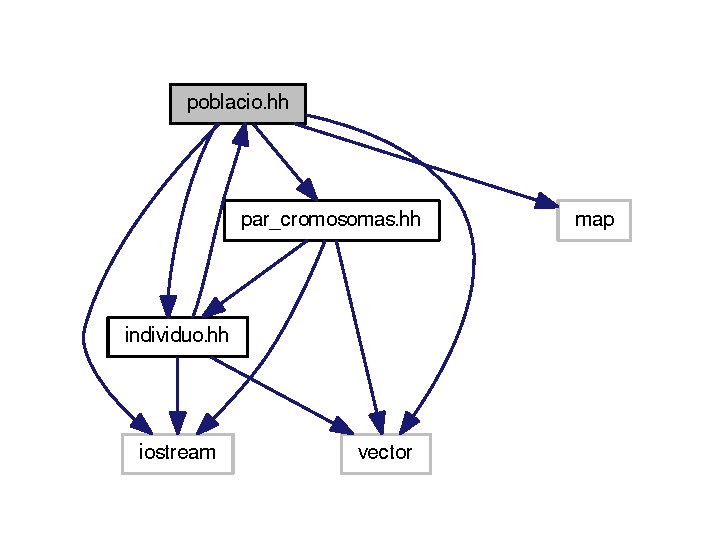
\includegraphics[width=343pt]{poblacio_8hh__incl}
\end{center}
\end{figure}
\subsection*{Clases}
\begin{DoxyCompactItemize}
\item 
class \hyperlink{class_poblacio}{Poblacio}
\end{DoxyCompactItemize}


\subsection{Descripción detallada}
Classe \hyperlink{class_poblacio}{Poblacio}. 


%--- End generated contents ---

% Index
\backmatter
\newpage
\phantomsection
\clearemptydoublepage
\addcontentsline{toc}{chapter}{Índice}
\printindex

\end{document}
